\documentclass[crop, tikz]{standalone}
\usepackage{tikz}

\usetikzlibrary{arrows,shapes, decorations.pathmorphing,backgrounds,positioning}
\usetikzlibrary{decorations.pathreplacing}
\usetikzlibrary{arrows.meta}

\tikzstyle{smallnode}=[draw, circle, inner sep=2pt]
\tikzstyle{stateTransition}=[->, thick, -{Latex[length=2mm,width=2mm]}]


\begin{document}
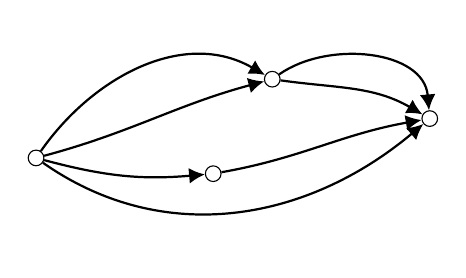
\begin{tikzpicture}
    \node[smallnode] (n0) at (-3, -1) {};
    \node[smallnode] (n1) at (-0.75, -1.2) {};
    \node[smallnode] (n2) at (0, 0) {};
    \node[smallnode] (n3) at (2, -0.5) {};
    
    % Arcs
    \draw[stateTransition] (n0) to[out=15,in=195] node [midway, sloped, above] {} (n2);
    \draw[stateTransition] (n0) to[out=55,in=150] node [midway, sloped, above] {} (n2);
    \draw[stateTransition] (n0) to[out=-15,in=185] node [midway, sloped, above] {} (n1);
    \draw[stateTransition] (n0) to[out=-35,in=220] node [midway, sloped, above] {} (n3);
    \draw[stateTransition] (n1) to[out=10,in=190] node [midway, sloped, below] {} (n3);
    \draw[stateTransition] (n2) to[out=35,in=95] node [midway, sloped, below] {} (n3);
    \draw[stateTransition] (n2) to[out=352,in=150] node [midway, sloped, above] {} (n3);

\end{tikzpicture}

\end{document}